\section{Appendix}

\subsection{Q5: Test result's confusion matrix and success/failure cases }
\label{subsec:Q5-1}
The optimal parameters determined for the random forest through experiments are $N=250$, $D=8$, and $\text{splitnum}=10$. With this configuration, each real-time executable weak learner—axis-aligned and two-pixel tests—each was trained 10 times. The confusion matrix results below represent the best test accuracy among the 10 repetitive train results.

\begin{figure}[h]
	\centering
	\begin{subfigure}[t]{0.4\linewidth}
		\centering
		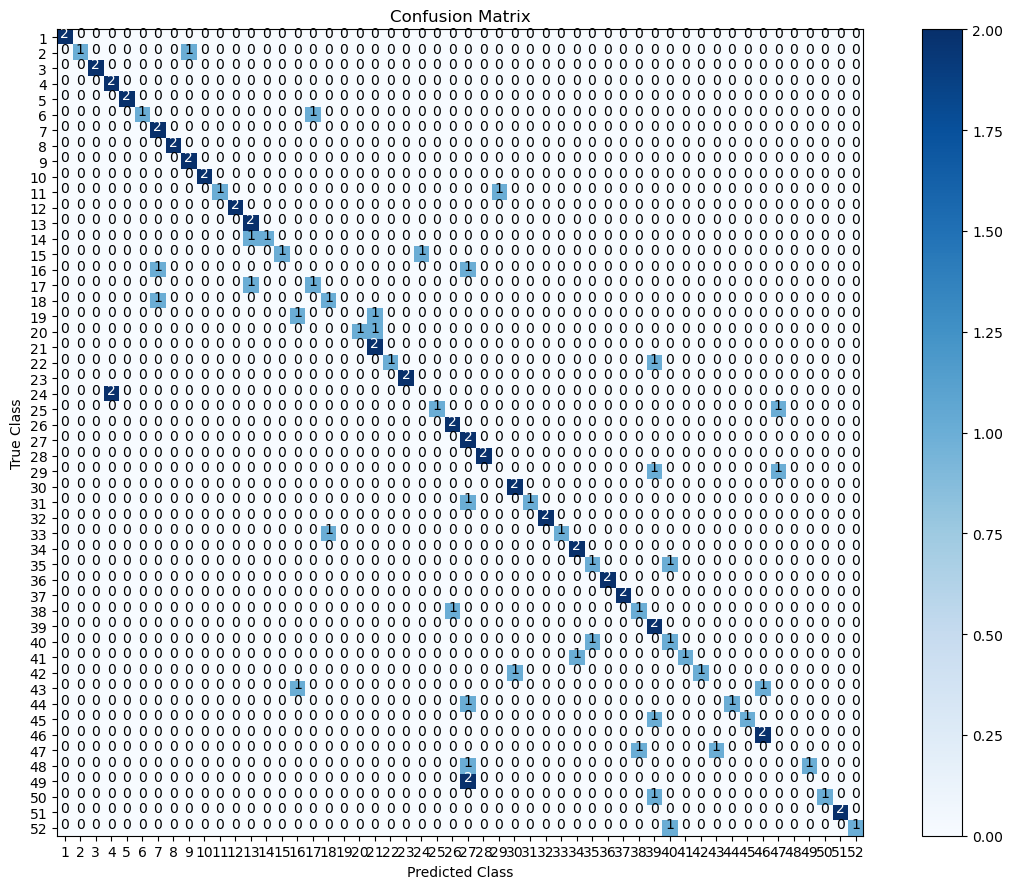
\includegraphics[width=\linewidth]{image/q5-fig6.png}
		\caption{Axis-aligned weak learner, test accuracy=0.644}
		\label{fig:q5-fig6}
	\end{subfigure}%
	\quad
	\begin{subfigure}[t]{0.4\linewidth}
		\centering
		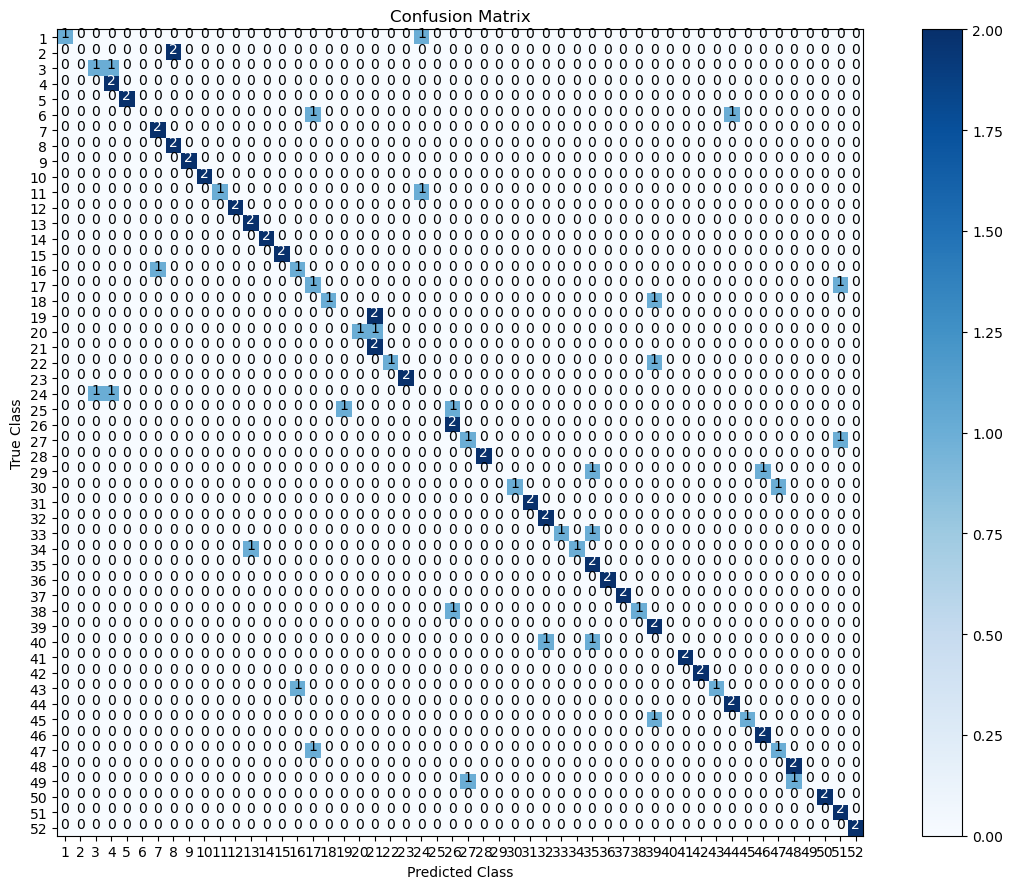
\includegraphics[width=\linewidth]{image/q5-fig8.png}
		\caption{Two-pixel test weak learner, test accuracy=0.692}
		\label{fig:q5-fig8}
	\end{subfigure}
	\caption{Confusion matrix of optimal cases ($N=250$, $D=8$, and $\text{splitnum}=10$)}
\end{figure}

Additionally, the example success and failure cases based on the confusion matrix results above are shown below. Compared to the success cases, the failure cases show a higher similarity between the failed image and the predicted class, meaning that our model is reasonable.
\begin{figure}
	\centering
	\begin{subfigure}{0.45\linewidth}
		\centering
		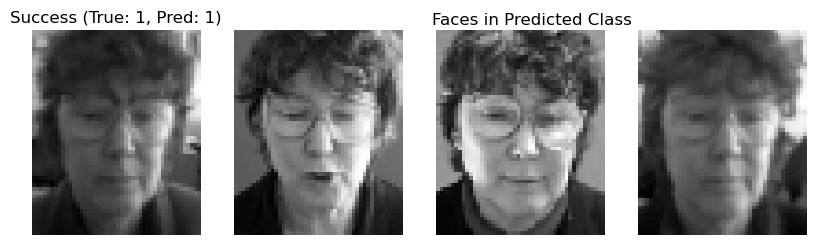
\includegraphics[width=\linewidth]{image/q5-app/q5-axis-succ1.png}
	\end{subfigure}%
	\quad
	\begin{subfigure}{0.45\linewidth}
		\centering
		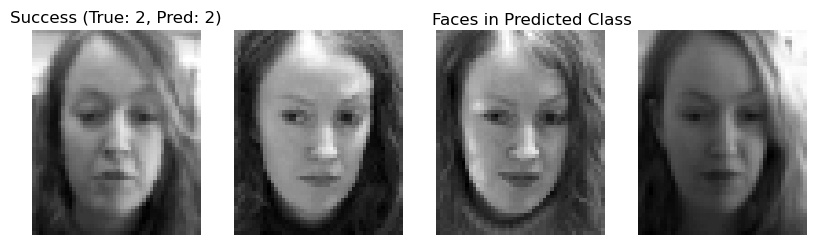
\includegraphics[width=\linewidth]{image/q5-app/q5-axis-succ2.png}
	\end{subfigure}
	\caption{Axis-aligned weak learner: Example success case}
\end{figure}
\begin{figure}
	\centering
	\begin{subfigure}[t]{0.45\linewidth}
		\centering
		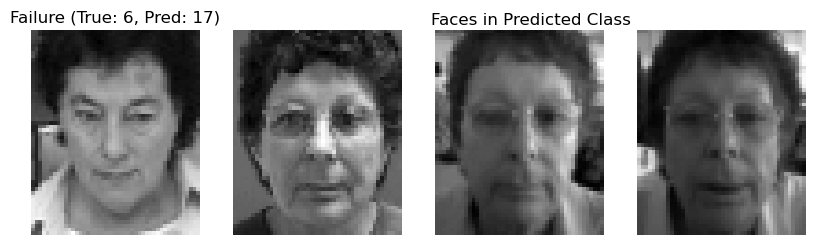
\includegraphics[width=\linewidth]{image/q5-app/q5-axis-fail1.png}
	\end{subfigure}%
	\quad
	\begin{subfigure}[t]{0.45\linewidth}
		\centering
		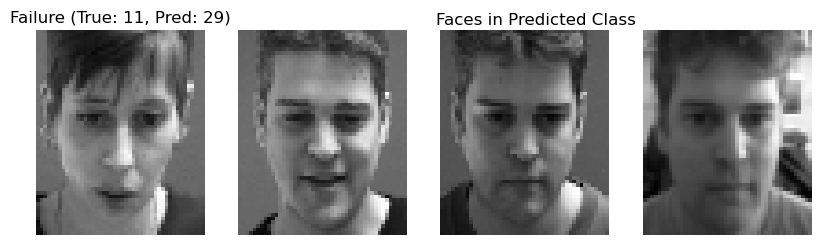
\includegraphics[width=\linewidth]{image/q5-app/q5-axis-fail2.png}
	\end{subfigure}
	\caption{Axis-aligned weak learner: Example failure case}
\end{figure}

\begin{figure}
	\centering
	\begin{subfigure}{0.45\linewidth}
		\centering
		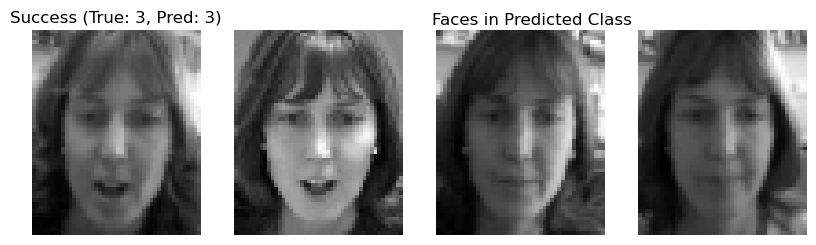
\includegraphics[width=\linewidth]{image/q5-app/q5-two-succ1.png}
	\end{subfigure}%
	\quad
	\begin{subfigure}{0.45\linewidth}
		\centering
		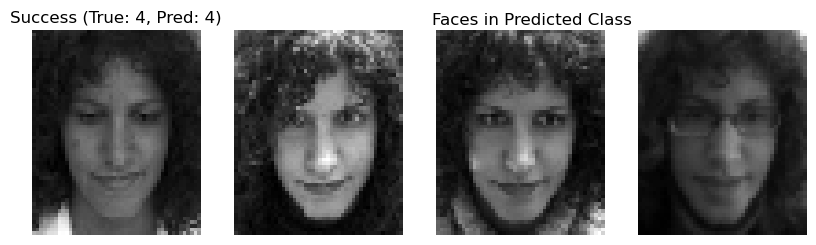
\includegraphics[width=\linewidth]{image/q5-app/q5-two-succ2.png}
	\end{subfigure}
	\caption{Two-pixel test weak learner: Example success case}
\end{figure}
\begin{figure}
	\centering
	\begin{subfigure}{0.45\linewidth}
		\centering
		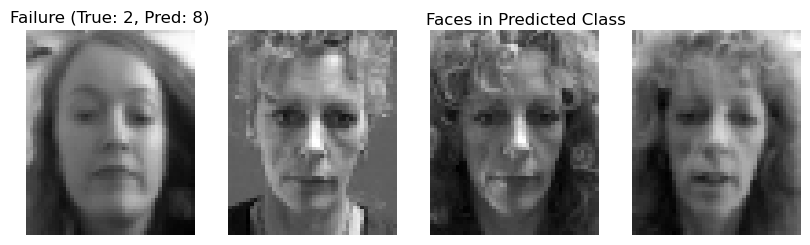
\includegraphics[width=\linewidth]{image/q5-app/q5-two-fail1.png}
	\end{subfigure}%
	\quad
	\begin{subfigure}{0.45\linewidth}
		\centering
		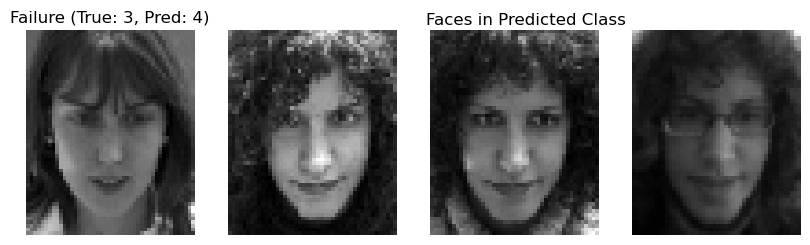
\includegraphics[width=\linewidth]{image/q5-app/q5-two-fail2.png}
	\end{subfigure}
	\caption{Two-pixel test weak learner: Example failure case}
\end{figure}

\subsection{Q5: Visualization of random forest's information gain process}
\label{subsec:Q5-2}